% Universidade Aberta
% Template TeX para relatório de trabalhos
% 2025
%
%
% Dados para a capa
\newcommand{\Titulo}{Planeamento e Desenvolvimento de Sistemas de Informação}
\newcommand{\SubTitulo}{Trabalho Grupo - Topico 5}
\newcommand{\Ano}{2025}
\newcommand{\Autor}{
    Pedro Morais - 2401849 \\
    Hugo Gonçalves - 2100562 \\
    Pedro Moro - 2001642 \\
    Luis Peixoto - 2402741 \\
}
%
%
\documentclass[12pt,a4paper,final]{article}
\usepackage{csquotes}
\usepackage{float}
\usepackage[portuguese]{babel}
\usepackage{polyglossia}
\usepackage{longtable}
\setdefaultlanguage{portuguese}
\usepackage{graphicx}
\graphicspath{ {./images/} }
\usepackage[a4paper,top=3cm,bottom=3cm,left=3.5cm,right=2cm]{geometry}
\usepackage{booktabs}
\setmainfont{Times New Roman}
\defaultfontfeatures{Ligatures=TeX}
\usepackage[pdfauthor=\Autor,
    pdftitle=\Titulo,
    colorlinks=true,
    linkcolor=black,
    citecolor=black,
    bookmarksopen=true]{hyperref}
\hypersetup{colorlinks, citecolor=black, urlcolor=black}
\usepackage{bookmark}
\usepackage[style=apa, backend=biber, sortcites, url=true, language=portuguese]{biblatex}
\usepackage{fontspec}
\DeclareLanguageMapping{portuguese}{portuguese-apa}
\addbibresource{ref.bib}
\renewcommand{\baselinestretch}{1.5}
\begin{document}
    \title{\Titulo}
    \author{\Autor}
    \date{\Ano}
    \pagenumbering{gobble}
    \begin{titlepage}
        \begin{center}
            \vspace*{4cm}

            \textbf{\large UNIVERSIDADE ABERTA}

            \textbf{\large UNIVERSIDADE DE TRÁS-OS-MONTES E ALTO DOURO}

            \vspace{1cm}

            \begin{minipage}{0.4\textwidth}
                \centering
                
\includegraphics[width=0.8\textwidth]{uab}
            \end{minipage}
            \begin{minipage}{0.4\textwidth}
                \centering
                
\includegraphics[width=0.8\textwidth]{utad}
            \end{minipage}

            \vspace{1.5cm}

            \textbf{\large \Titulo}

            \textbf{\large \SubTitulo}

            \vspace{1.5cm}

            \textbf{\large \Autor}

            \vspace{2cm}

            \textbf{\large Mestrado em Engenharia Informática e Tecnologia Web}
            \vfill
            \textbf{\Ano}
        \end{center}
    \end{titlepage}
    \renewcommand{\contentsname}{Índice}
    \cleardoublepage
    \pagenumbering{roman}
    \tableofcontents
    \newpage
    \listoffigures
    \newpage
    \cleardoublepage
    \pagenumbering{arabic}

    \section*{Q7 - Sumário das Entidades de Informação da DMHU}
    \addcontentsline{toc}{section}{Q7 - Sumário das Entidades de Informação da DMHU}

    Conforme o feedback anterior e no contexto da transformação digital da Direção Municipal de Higiene Urbana (DMHU), tornou-se essencial mapear e classificar todas as entidades de informação que suportam os seus processos operacionais e estratégicos.
    Esta fase do trabalho dedica-se à identificação exaustiva dessas entidades, bem como à sua respetiva classificação segundo o modelo proposto por William H. Inmon, referência incontornável na área dos armazéns de dados.

    De forma a garantir uma arquitetura de dados robusta, escalável e preparada para integração com soluções de \textit{Business Intelligence} e \textit{Smart City}, foi adotada uma abordagem tripla para a classificação das entidades informacionais:
    \begin{itemize}
        \item \textbf{Tipo de Origem:} distingue entre \textit{Entidades Primitivas}, diretamente recolhidas a partir das fontes operacionais, e \textit{Entidades Derivadas}, construídas por transformação, agregação ou combinação de outras entidades.
        \item \textbf{Temporalidade:} classifica os dados como \textit{Históricos}, quando mantêm versões ao longo do tempo, \textit{Projetados}, quando são usados para simulações e planeamento, ou \textit{Referenciais}, quando são catálogos ou listas estáticas.
        \item \textbf{Acesso:} identifica se os dados são \textit{Públicos} (disponíveis para consumo externo) ou \textit{Privados} (uso interno à organização).
    \end{itemize}

    Com base nestes critérios, foi elaborada uma tabela que representa a visão consolidada das entidades informacionais da DMHU. Esta tabela visa colmatar lacunas de versões anteriores, incluindo agora todas as identidades envolvidas na operação e gestão da higiene urbana da cidade de Lisboa — assegurando assim a completude e rastreabilidade necessárias à implementação de um verdadeiro armazém de dados corporativo.

    A Tabela~\ref{tab:inmon} apresenta essa classificação detalhada.

    \renewcommand{\arraystretch}{1.3}
    \begin{longtable}{|p{6cm}|p{7cm}|}
        \caption{Classificação Inmon das entidades de informação da DMHU}
        \label{tab:inmon} \\
        \hline
        \textbf{Entidade Informacional}          & \textbf{Classificação Inmon}    \\
        \hline
        \endfirsthead

        \hline
        \textbf{Entidade Informacional}          & \textbf{Classificação Inmon}    \\
        \hline
        \endhead

        \hline
        \endfoot

        Cidadão                                  & Primitiva, Histórica, Pública   \\
        Ocorrência                               & Primitiva, Histórica, Pública   \\
        Pedido de Assistência                    & Derivada, Histórica, Pública    \\
        Folha de Inquérito                       & Derivada, Histórica, Privada    \\
        Resposta de Serviço                      & Derivada, Histórica, Privada    \\
        Resposta Associada                       & Derivada, Histórica, Privada    \\
        Endereço                                 & Primitiva, Histórica, Pública   \\
        Equipamento de Deposição                 & Primitiva, Histórica, Pública   \\
        Local de Contentor                       & Primitiva, Projetada, Pública   \\
        Circuito de Recolha                      & Primitiva, Projetada, Pública   \\
        PRS (Ponto de Recolha Seletiva)          & Primitiva, Histórica, Pública   \\
        Área de Apoio                            & Primitiva, Projetada, Privada   \\
        Local de Descarga                        & Primitiva, Projetada, Pública   \\
        Requisição ao Armazém                    & Derivada, Histórica, Privada    \\
        Bem Móvel / Stock                        & Primitiva, Histórica, Privada   \\
        Funcionário (Colaborador)                & Primitiva, Histórica, Privada   \\
        Frequência/Formação                      & Derivada, Histórica, Privada    \\
        Curso de Formação                        & Primitiva, Projetada, Privada   \\
        Uniforme                                 & Primitiva, Projetada, Privada   \\
        Equipamento de Proteção Individual       & Primitiva, Projetada, Privada   \\
        Equipamento (Máquinas)                   & Primitiva, Histórica, Privada   \\
        Veículo                                  & Primitiva, Histórica, Privada   \\
        Movimento de Equipamento                 & Derivada, Histórica, Privada    \\
        Garage                                   & Primitiva, Projetada, Privada   \\
        Tipo de Máquina                          & Primitiva, Referencial, Pública \\
        Oficina                                  & Primitiva, Projetada, Privada   \\
        Plano de Manutenção                      & Derivada, Projetada, Privada    \\
        Inspeção                                 & Derivada, Histórica, Privada    \\
        Evento (ação pública)                    & Derivada, Histórica, Pública    \\
        Reclamação                               & Primitiva, Histórica, Pública   \\
        Sugestão                                 & Primitiva, Histórica, Pública   \\
        Pedido de Recolha Volumosa               & Derivada, Histórica, Pública    \\
        Pedido de Controlo de Pragas             & Derivada, Histórica, Pública    \\
        Pedido de Contentor                      & Derivada, Histórica, Pública    \\
        Pedido de Intervenção                    & Derivada, Histórica, Pública    \\
        Pedido de Evento                         & Derivada, Histórica, Pública    \\
        Avaliação de Desempenho                  & Derivada, Histórica, Privada    \\
        Atestado de Aptidão Médica               & Primitiva, Histórica, Privada   \\
        Acidente de Trabalho                     & Primitiva, Histórica, Privada   \\
        Ausência/Assiduidade                     & Derivada, Histórica, Privada    \\
        Registo de Frequência (Relógio de Ponto) & Primitiva, Histórica, Privada   \\
        Responsável de Circuito/Operação         & Primitiva, Histórica, Privada   \\
    \end{longtable}

    \section*{Q9 - Arquitetura de Aplicações AS-IS (Application Structure)}
    \addcontentsline{toc}{section}{Q9 - Arquitetura de Aplicações AS-IS}

    A arquitetura de aplicações AS-IS da Direção Municipal de Higiene Urbana (DMHU) é caracterizada por uma elevada heterogeneidade tecnológica e por uma forte dependência de sistemas desenvolvidos internamente.
    A estrutura de aplicações revela fragmentação e sobreposição funcional, refletindo um crescimento orgânico das soluções ao longo do tempo, com fraca integração.

    A Figura~\ref{fig:q9-as-is-structure} apresenta a arquitetura de aplicações AS-IS da DMHU, segundo o ponto de vista de \textbf{Application Structure} do ArchiMate.
    Foram identificados cinco grandes domínios funcionais, cada um suportado por um conjunto distinto de aplicações:

    \begin{itemize}
        \item \textbf{Gestão da Higiene Urbana e Recolha de Resíduos} – LU, LU\_SIG, Bee2Waste, Paper Bins, Pigeons.
        \item \textbf{Gestão de Recursos Humanos} – RH2011, Relógio Ponto, SST (em migração para Oracle APEX).
        \item \textbf{Gestão da Frota e Oficinas} – GIF, Municipal Fleet, Cartrack.
        \item \textbf{Gestão de Interação com o Munícipe} – NaMinhaRuaLX (GOPI), LxRequests.
        \item \textbf{Gestão de Armazém e Equipamento} – Stocks, SAP\_SRM, SAP\_Finanças.
    \end{itemize}

    As aplicações estão, na sua maioria, implementadas como \textit{desktop applications}, desenvolvidas com tecnologias Windows Forms e VB.NET, com exceção de alguns módulos Web e mobile.
    Esta estrutura levanta desafios de manutenção, escalabilidade e integração com plataformas modernas.

    \vspace{0.5cm}
    \begin{figure}[H]
        \centering
        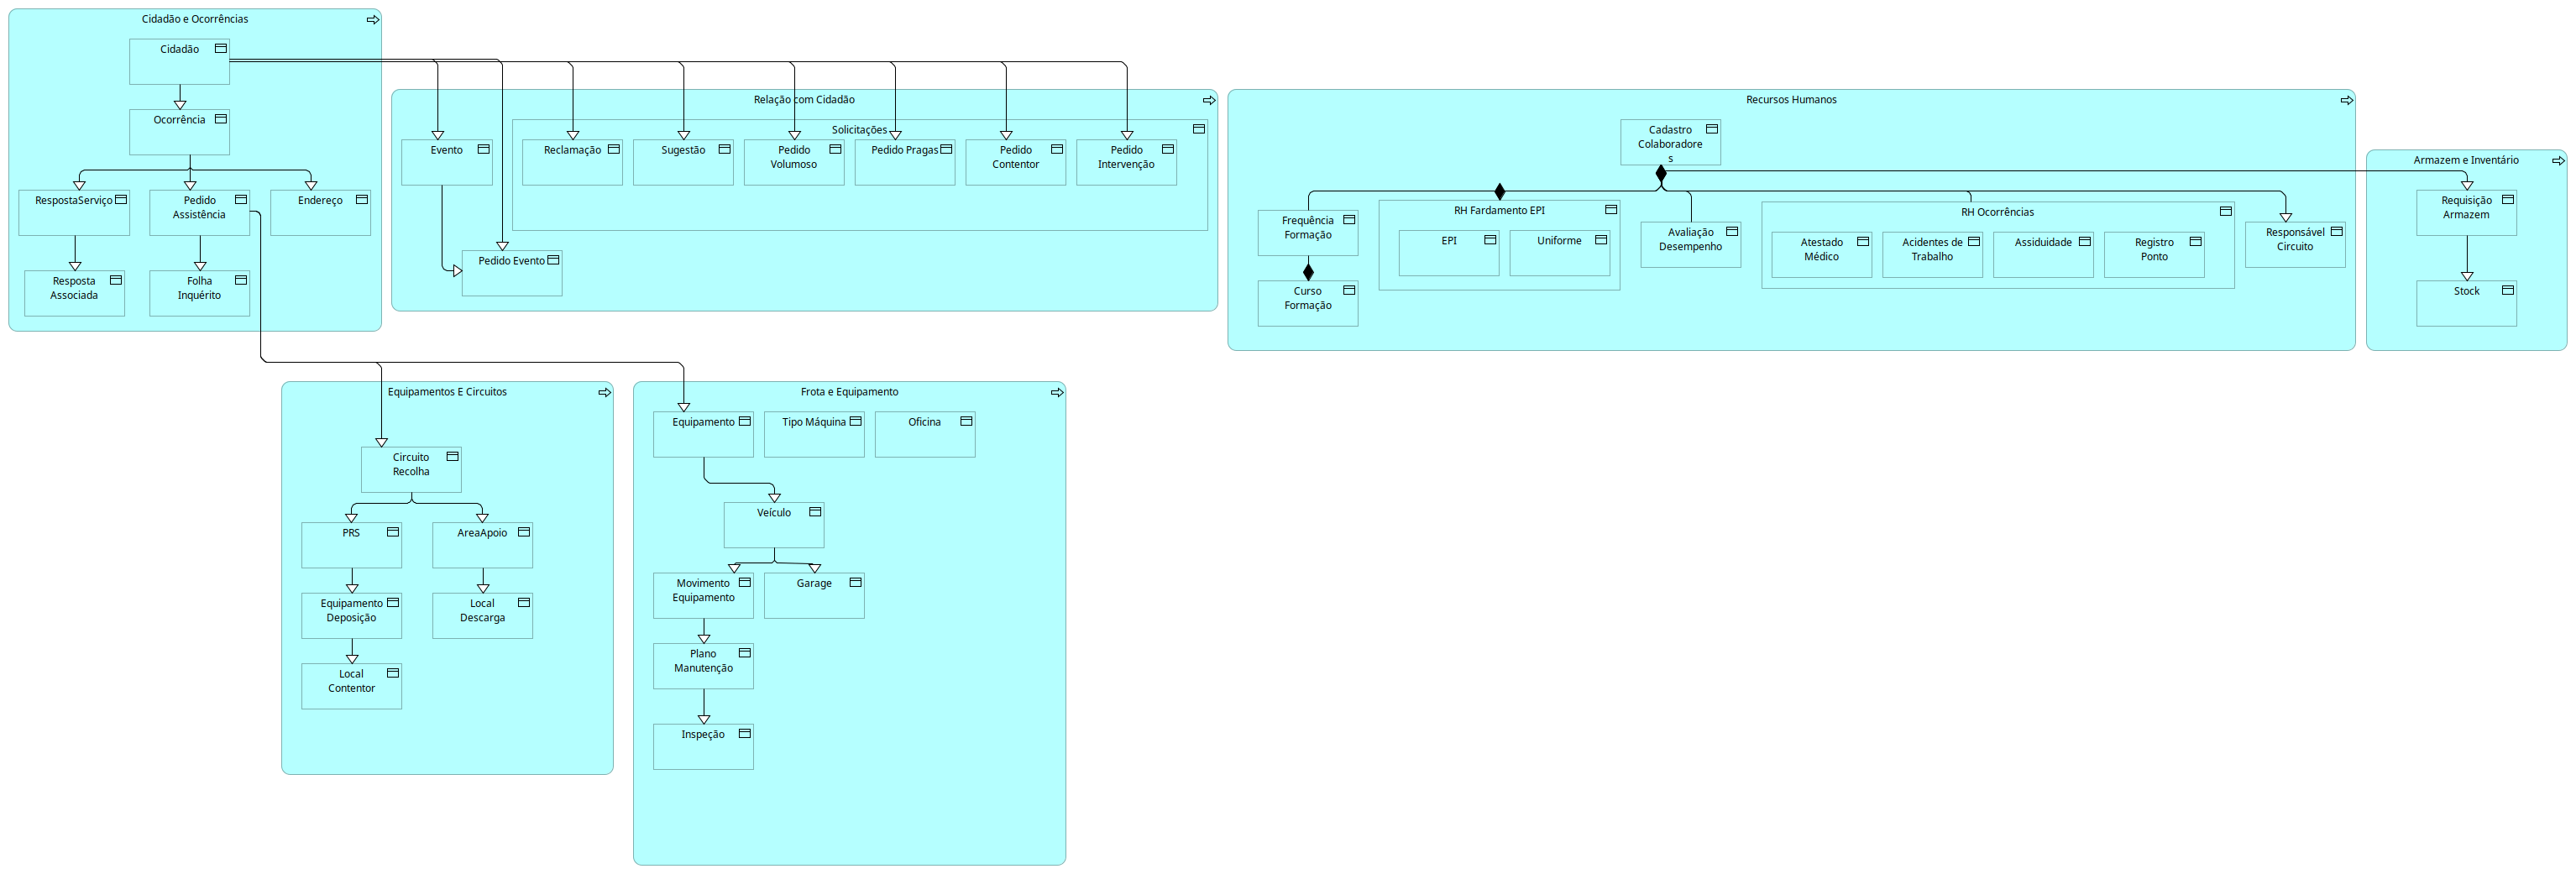
\includegraphics[width=\textwidth]{Q9}
        \caption{Arquitetura de Aplicações AS-IS – Estrutura das Aplicações da DMHU}
        \label{fig:q9-as-is-structure}
    \end{figure}

    \section*{Q10 - Arquitetura de Aplicações AS-IS (Application Usage)}
    \addcontentsline{toc}{section}{Q10 - Arquitetura de Aplicações AS-IS (Application Usage)}

    A arquitetura de utilização das aplicações da Direção Municipal de Higiene Urbana (DMHU) evidencia uma forte especialização por domínio funcional. A abordagem adotada no levantamento e modelação procurou evidenciar as relações de suporte entre as funções de negócio e os sistemas atualmente em uso, de acordo com a perspetiva de \textbf{Application Usage}, segundo o ArchiMate 3.0.

    As aplicações existentes estão organizadas por áreas-chave, com destaque para:

    \begin{itemize}
        \item \textbf{Gestão de Resíduos e Equipamentos} – LU, Bee2Waste, Scale, Paper Bins Management e Pigeons Management dão suporte à gestão e execução de circuitos, bem como à monitorização de ativos.
        \item \textbf{Gestão de Recursos Humanos} – RH2011, Relógio Ponto, SST e Accidents Management cobrem desde o cadastro de colaboradores até à avaliação de desempenho e gestão de ausências.
        \item \textbf{Gestão da Frota} – GIF (EAM e Database Link), Cartrack API e Viatura suportam todo o ciclo de vida dos veículos, da aquisição ao abate.
        \item \textbf{Relacionamento com o Cidadão} – NaMinhaRuaLX (GOPI) e LxRequests garantem o registo e tratamento de ocorrências, reclamações, elogios e pedidos de informação.
        \item \textbf{Gestão de Armazém e Consumíveis} – Stocks e SAP SRM apoiam os pedidos internos de materiais e fardamento.
        \item \textbf{Operações Policiais e Controlo Municipal} – GIC, SF-PM, GML e Vehicle Park Management asseguram processos de inspeção, contraordenações e apreensão de veículos.
        \item \textbf{Outros domínios de suporte} – Incluem POIs, TNC, Projects, MeiosRec, SAP Finanças, SendMessages, entre outros, garantindo funções complementares como auditorias, gestão documental, comunicação interna e interação com parceiros.
    \end{itemize}

    As Figuras~\ref{fig:q10_1} a~\ref{fig:q10_8} apresentam a arquitetura de uso das aplicações, agrupadas por domínios funcionais.

    \vspace{0.5cm}

    \begin{figure}[H]
        \centering
        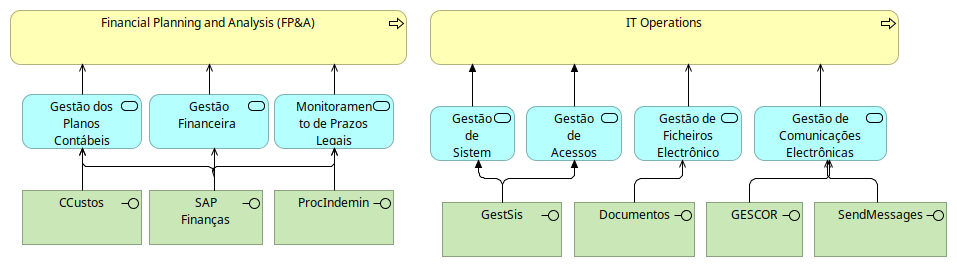
\includegraphics[width=\textwidth]{Q10_1}
        \caption{Application Usage – Gestão de Resíduos e Equipamento}
        \label{fig:q10_1}
    \end{figure}

    \begin{figure}[H]
        \centering
        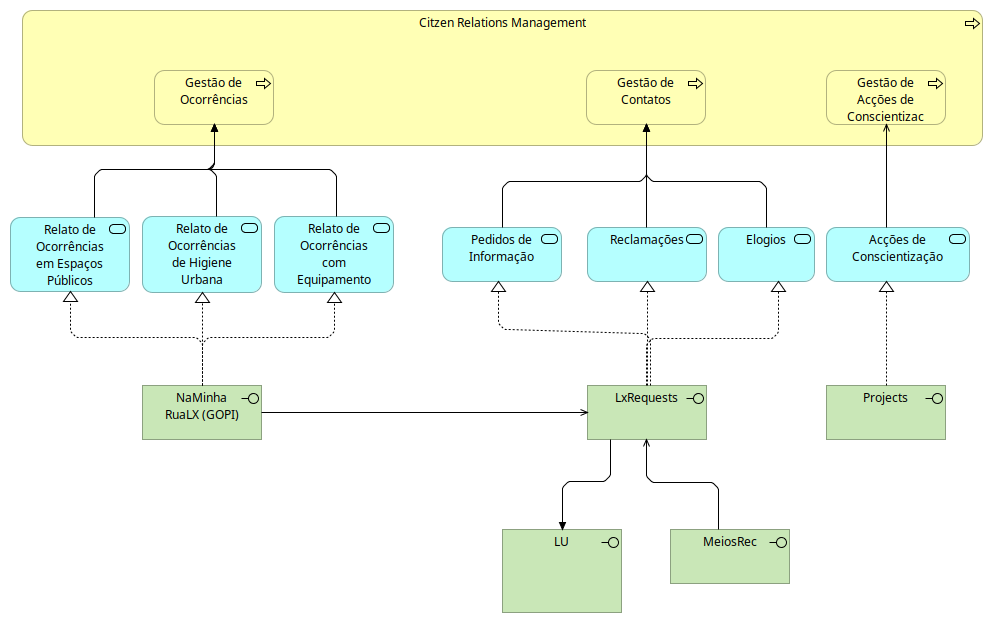
\includegraphics[width=0.6\textwidth]{Q10_2}
        \caption{Application Usage – Gestão de Armazém}
        \label{fig:q10_2}
    \end{figure}

    \begin{figure}[H]
        \centering
        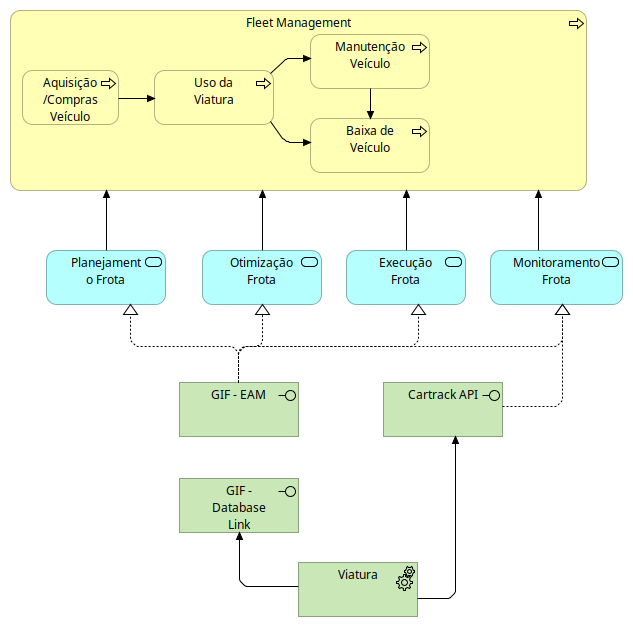
\includegraphics[width=\textwidth]{Q10_3}
        \caption{Application Usage – Ações da Polícia Municipal}
        \label{fig:q10_3}
    \end{figure}

    \begin{figure}[H]
        \centering
        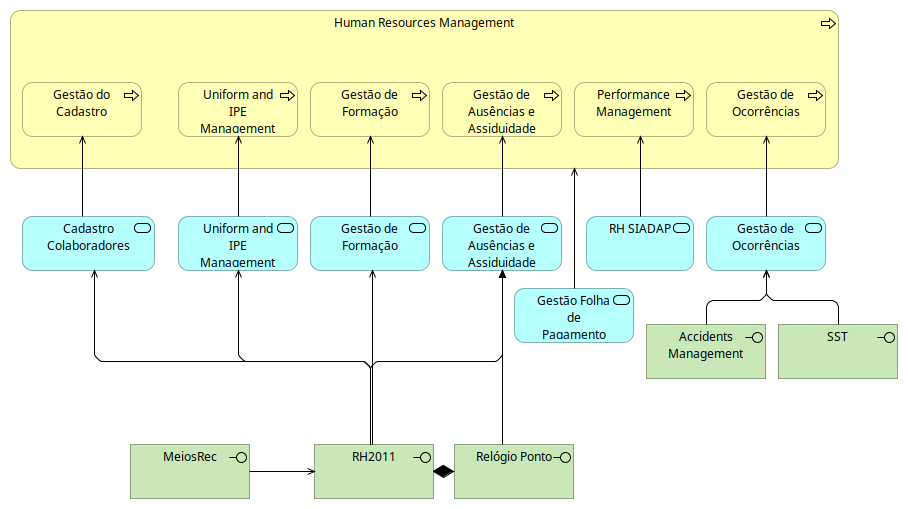
\includegraphics[width=\textwidth]{Q10_4}
        \caption{Application Usage – Gestão de Parceiros e Auditorias}
        \label{fig:q10_4}
    \end{figure}

    \begin{figure}[H]
        \centering
        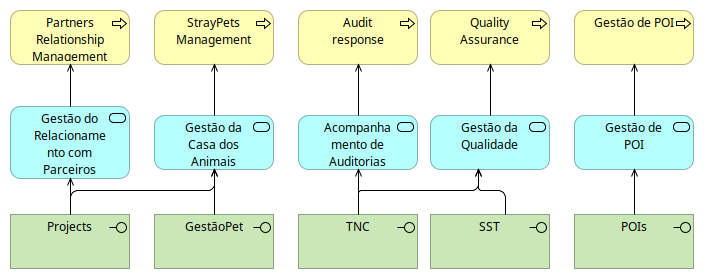
\includegraphics[width=\textwidth]{Q10_5}
        \caption{Application Usage – Gestão de Recursos Humanos}
        \label{fig:q10_5}
    \end{figure}

    \begin{figure}[H]
        \centering
        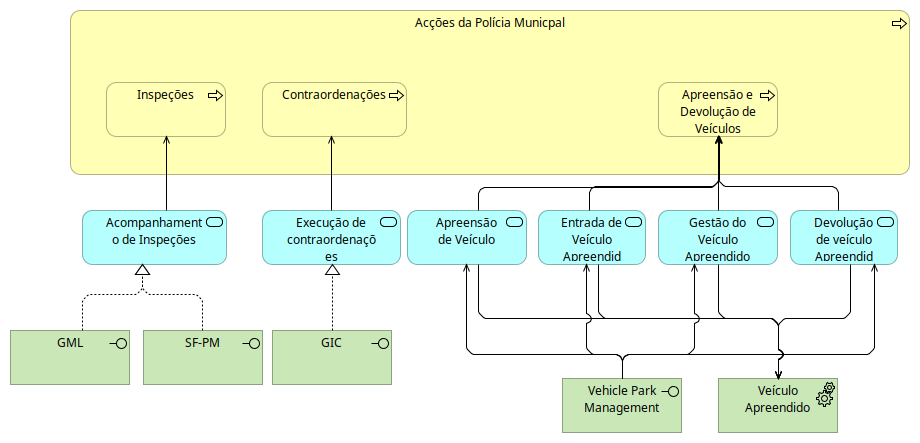
\includegraphics[width=0.9\textwidth]{Q10_6}
        \caption{Application Usage – Gestão de Frota}
        \label{fig:q10_6}
    \end{figure}

    \begin{figure}[H]
        \centering
        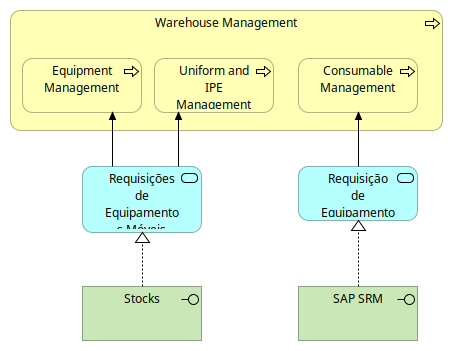
\includegraphics[width=\textwidth]{Q10_7}
        \caption{Application Usage – Gestão de Relação com o Cidadão}
        \label{fig:q10_7}
    \end{figure}

    \begin{figure}[H]
        \centering
        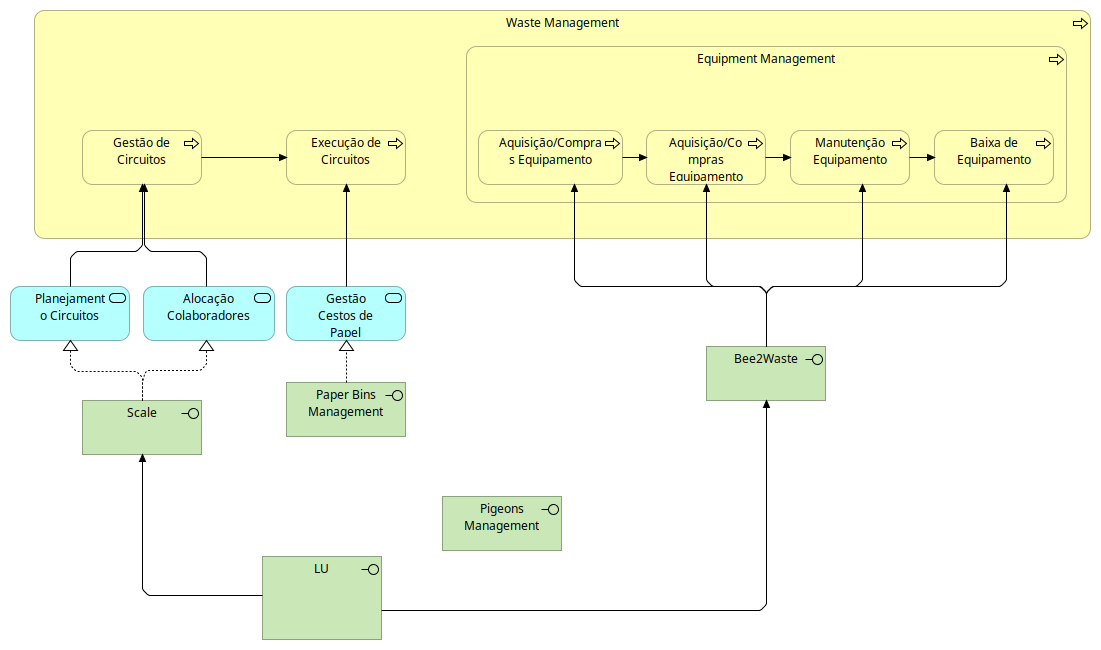
\includegraphics[width=\textwidth]{Q10_8}
        \caption{Application Usage – Gestão Financeira e TI}
        \label{fig:q10_8}
    \end{figure}

    \section*{Q13 - Matriz CRUD entre Entidades e Processos}
    \addcontentsline{toc}{section}{Q13 - Matriz CRUD entre Entidades e Processos}

    A matriz CRUD apresentada na folha de cálculo em anexo, relaciona os principais processos de negócio da DMHU com as respetivas entidades de informação envolvidas.

    Esta matriz permite identificar quais os processos que \textbf{criam (C)}, \textbf{lêem (R)}, \textbf{atualizam (U)} e \textbf{eliminam (D)} cada entidade, contribuindo para a clarificação de responsabilidades sobre os dados e a definição de zonas críticas de integração.
    Além disso, serve de base para iniciativas de melhoria contínua e racionalização de sistemas.

    \section*{Q14 - Matriz CRUD com Aplicações e Dependências (BSP)}
    \addcontentsline{toc}{section}{Q14 - Matriz CRUD com Aplicações e Dependências (BSP)}

    A Figura~\ref{fig:q14-domains} apresenta a representação dos domínios de informação identificados na DMHU, incluindo a decomposição das entidades por área funcional.
    Esta visão permite uma leitura mais clara das dependências de informação e constitui base para a análise CRUD entre aplicações.

    Complementarmente, a Tabela CRUD (ver ficheiro em anexo) mapeia as aplicações existentes aos processos e entidades, segundo a metodologia BSP (\textbf{Business}, \textbf{System}, \textbf{Program}). Esta análise permite:
    \begin{itemize}
        \item Identificar sobreposições funcionais e silos de informação;
        \item Determinar que aplicações suportam que operações CRUD sobre cada entidade;
        \item Priorizar oportunidades de integração, substituição ou consolidação.
    \end{itemize}

    \vspace{0.5cm}
    \begin{figure}[H]
        \centering
        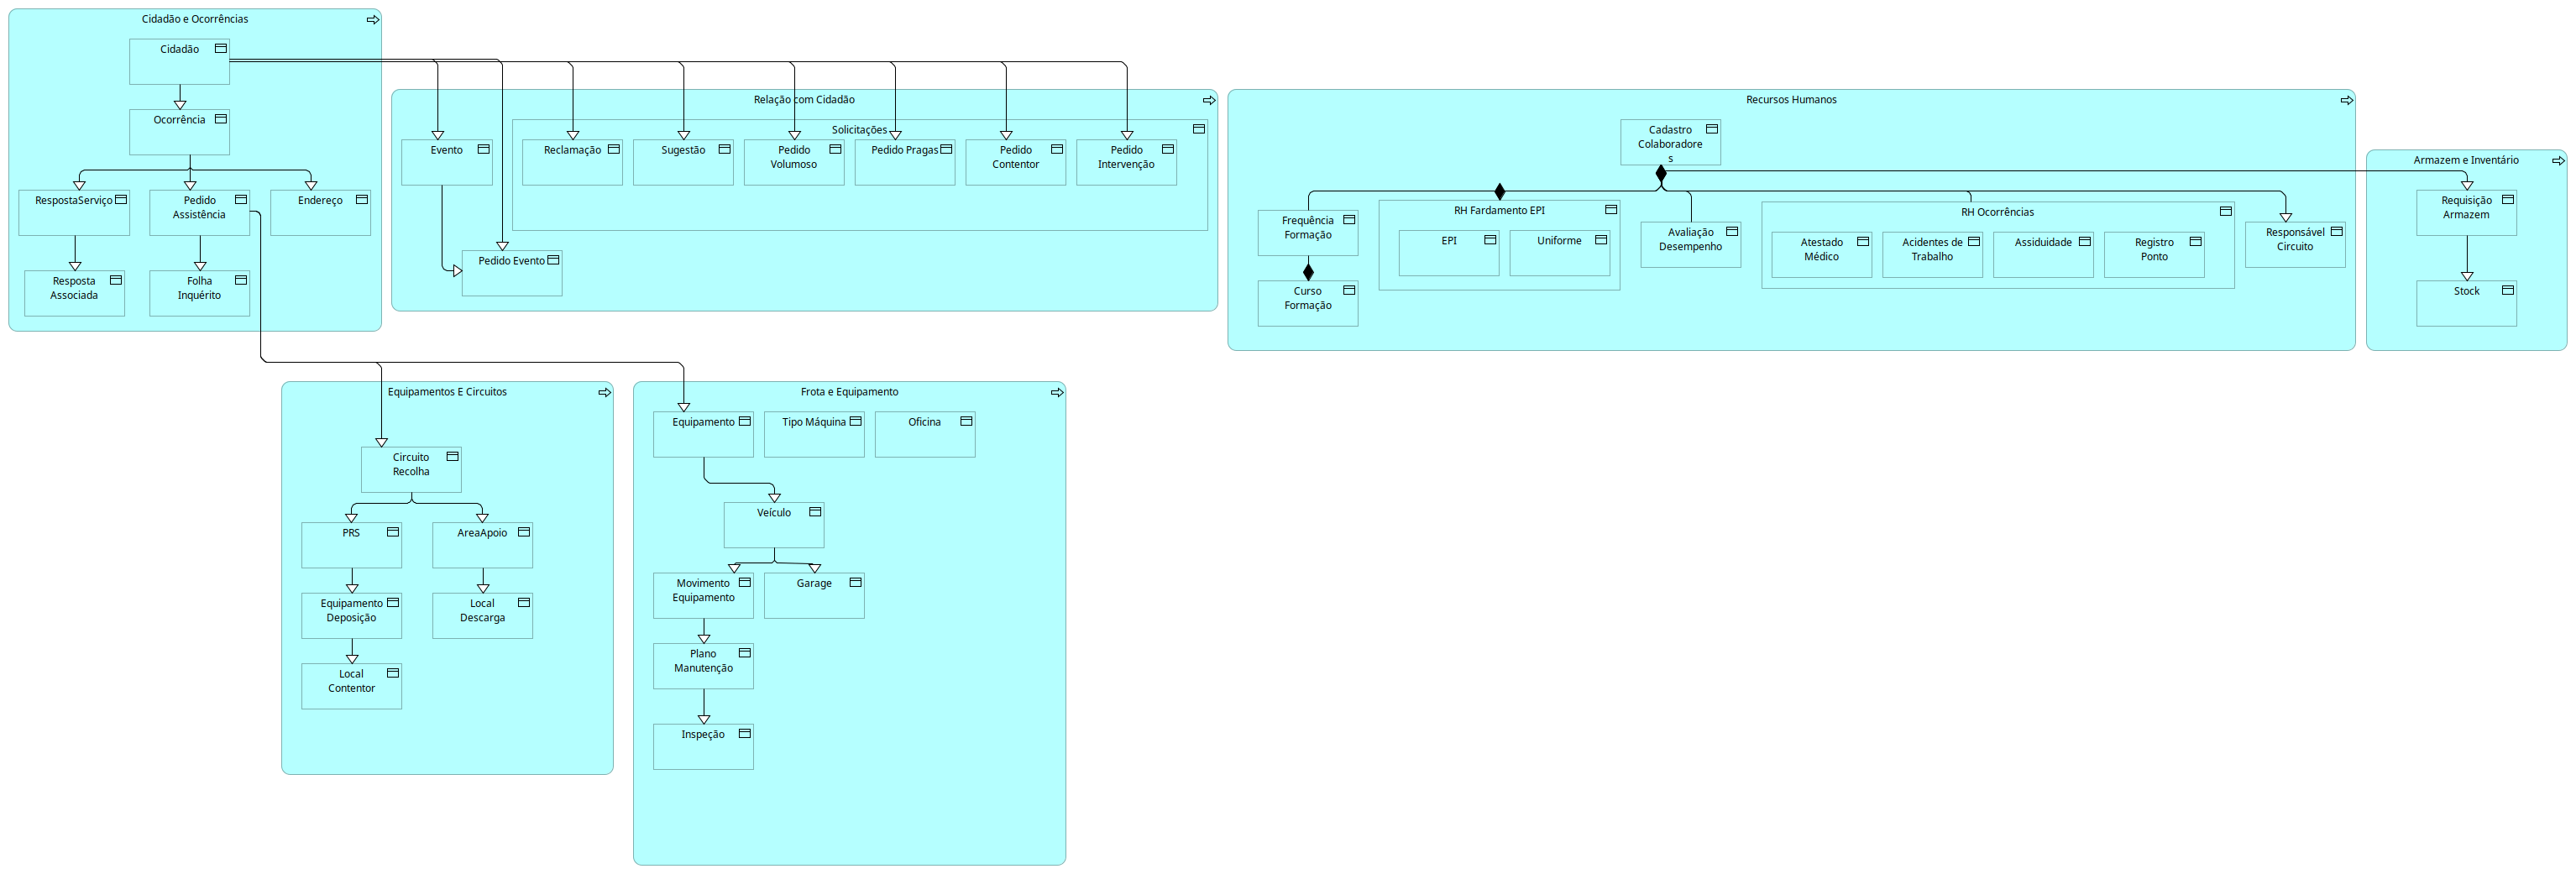
\includegraphics[width=\textwidth]{Q13}
        \caption{Domínios Informacionais e Entidades Relacionadas - Visão BSP}
        \label{fig:q14-domains}
    \end{figure}


    \newpage
    \nocite{*}
    \printbibliography
\end{document}